
\section{Ressourcen- und Speicher-Management}\label{sec:resourcenmanagement}

\renewcommand{\kapitelautor}{Autor: Marvin Kurka}

Kotlin, wie auch Java und andere JVM-basierende Sprachen verwendet einen Garbage Collector, kurz GC, um den
Speicherplatz von nicht mehr verwendetet Objekten freizugeben.\zit{oracleGC}

\subsection{Wie funktioniert Garbage Collection?}

Garbage Collection ist in zwei Phasen aufgeteilt.
In der ersten Phase, dem Marking, werden alle Objekte, für die noch eine Referenz existiert, markiert.
Dabei geht der GC von sogenannten Roots aus, was Objekte sind, auf die das Programm eine unmittelbare
Referenz hat.
Diese werden markiert und der Prozess wird rekursiv für alle Referenzen, die diese Objekte halten, wiederholt.
Am Ende sind alle Objekte, für die das Programm noch eine gültige Referenz hält markiert.
In der zweiten Phase werden alle Objekte, die nicht markiert wurden, und demnach nicht mehr erreichbar sind, gelöscht.
Zusätzlich kann hier eine Defragmentierung stattfinden.\zit{oracleGC}

Eine GC durchzuführen ist teuer.
Erst muss jedes Objekt in der Baumstruktur des Heaps durchgegangen und markiert werden, und dann beim
Löschen/Defragmentieren müssen große Teile des Heaps kopiert werden.
Dazu kommt, dass es sich bei Garbage Collections um "Stop the World Events" handelt.
Da große Teile des GC-Prozesses nicht parallel mit den Application Threads laufen können, muss das
Programm für die Dauer der Garbage Collection pausiert werden, was sowohl die Geschwindigkeit als auch die
Responsiveness des Programms beeinträchtigt.\zit{oracleGC}

Um dieses Problem wenigstens zu mindern, verwendet die JVM eine generational Garbage Collection.
Die meisten Objekte, die in der Laufzeit eines Programms allokiert werden, haben nur eine sehr geringe Lebenszeit,
während einige wenige Objekte signifikant längere Lebenszeiten haben.
Die JVM macht sich das zu Nutze, um den Heap in verschiedene Generation einzuteilen, je nachdem wie viele GCs
ein Objekt schon überlebt hat.
Bei einem Minor Garbage Collection Event werden dann nur die jüngeren Generationen durchsucht, während bei einem
Major Garbage Collection Event der gesamte heap durchsucht wird.\zit{oracleGC}

\subsection{Gargabe Collection in Videospielen}

GC funktioniert am besten mit kleinen Objekten mit kurzer Lebensdauer.
Diese überleben im Idealfall schon die erste minor GC nicht, und müssen deshalb nicht in den Bereich der older
Generation überführt werden.
Außerdem ist das allokieren/kopieren/löschen durch die kleine Größe wenig Aufwand.
Weiters sollten große Objekte im Idealfall nicht im stable State des Programmes allokiert werden, um die Zahl an major
GCs gering zu halten.\zit{infoqJavaPerformance}

Allerdings ist es gerade in Videospielen so, dass es besonders viele sehr große und langlebige Objekte gibt.
Texturen, Animationen und Sounds können oft Megabytes an RAM benötigen und werden oft im stable state des Programms
allokiert, \zB bei einer Screen-Transition.
In Videospielen spielt oft auch die Latenz, also wie schnell auf User-Input reagiert wird, eine wichtige Rolle.
Diese kann durch GC beeinträchtigt werden, da diese die Applikation Thread pausiert und diese dann nicht sofort auf
den Input reagieren könne.

Außerdem werden oft Ressourcen verwendet, die gar nicht von einer konventionellen GC verwaltet werden können, da sie zur
GPU hochgeladen werden müssen.
Das inkludiert \zB Texturen oder Shader.
Solche Ressourcen könnten theoretisch über einen Finalizer, der automatisch läuft, bevor die GC ein Objekt collected,
freigegeben werden, das würde die Performance des GC-Prozesses allerdings weiter verschlechtern.\zit{infoqJavaPerformance}

Ein weiterer Grund, warum man sich bei großen Objekten nicht auf den GC verlassen sollte, ist, dass oft eine feine
Kontrolle über große Ressourcen notwendig ist.
Sollte irgendwo im Programm noch eine einzelne Referenz zu einem Objekt existieren, wird dieses nicht vom GC
eingesammelt, auch wenn es vielleicht nicht mehr verwendet wird.
So können sehr einfach Memory Leaks entstehen, die auch noch sehr schwer zu debuggen sind.
All das macht GC besonders ungeeignet für Videospiele und ist er Grund, warum LibGdx einen anderen Ansatz für das
Managen von großen Ressourcen verfolgt.

\subsection{LibGdx und das Disposable-Interface}

In LibGdx werden große Ressourcen durch nativen Code allokiert und nicht vom GC verwaltet.
Klassen, die solche Ressourcen repräsentieren, implementieren das Disposable-Interface, das die
\inlineKotlin{Disposable::dispose} Funktion zur Verfügung stellt.
Diese muss am Ende des Lebenszyklus des Objektes aufgerufen werden, um den allokierten Speicher wieder freizugeben.\zit{libGdxMemoryManagement}

Diese Herangehensweise macht den effizienten Umgang mit Ressourcen möglich und gibt dem Programmierer Kontrolle über
die Lebenszeit von großen Objekten.
Allerdings führt das auch dazu, dass viele Fehlerquellen, die durch GC eliminiert wurden, wieder auftreten können.
Beispiele sind Memory Leaks, die auftreten, wenn eine Ressource nicht wieder freigegeben wird, oder eine
Use-after-Free-Situation, bei der eine Ressource verwendet wird, obwohl sie eigentlich schon freigegeben wurde, was
zu undefinierten Verhalten führt.\zit{libGdxMemoryManagement}

\subsection{Der ResourceManager}

Gutes Ressourcenmanagement ist in der Spielentwicklung extrem wichtig.
Schlechtes Management kann \zB zu langen Wartezeiten bei Screen-Transitions führen, und so die Immersion brechen.
Aber falscher Umgang mit Ressourcen kann nicht nur das Spielerlebnis verschlechtern, er kann das Spiel sogar
komplett unspielbar machen.
Die im vorherigen Absatz beschriebenen Bugs wie Use-after-Free oder Memory Leaks können zu Crashes oder anderen
Fehlverhalten des Spiels führen.
Deswegen war das Ressourcenmanagement bei der Entwicklung von \FF eine besonders große Herausforderung.
Um diese zu bewältigen wurde der ResourceManager entwickelt, eine Klasse, die Ressourcen über die gesamte
Applikation hinweg verwaltet.

\subsubsection{Grundfunktion des ResourceManager}

Klassen, die Ressourcen vom ResourceManager verwenden wollen, müssen das ResourceBorrower-Interface implementieren.
Dieses enthält keine Funktionen, es dient nur dem Zweck, dem Programmierer zu erinnern, dass diese Klasse Ressourcen
verwendet und diese auch zurückgeben muss.

Eine Klasse, die ResourceBorrower implementiert kann die \inlineKotlin{ResourceManager::borrow} Funktion verwenden,
um sich eine Ressource auszuborgen.
Die Ressource muss zu diesem Zeitpunkt nicht unbedingt geladen sein, sie wird nur als in Verwendung markiert.
Um die Ressource tatsächlich zu bekommen, wird die \inlineKotlin{ResourceManager::get} Funktion verwendet.
Spätestens zu diesem Zeitpunkt wird das Laden erzwungen.
Um die Ressource wieder zurückzugeben, wird die \inlineKotlin{ResourceManager::giveBack} Funktion verwendet.
Auch hier gilt wieder, dass ein Aufruf dieser Funktion nicht unbedingt zum Entladen der Ressource führen muss,
da auch ein zweiter Borrower sie noch verwenden könnte.

Diese zentrale Verwaltung ermöglicht effizientes Management der Ressourcen, da der ResourceManager zu jedem Zeitpunkt
über die Gesamtsituation im Programm Bescheid weiß.
Das ermöglicht es, dass doppelte Laden von Ressourcen oder das Entladen und sofortige neu Laden zu verhindern.

\subsubsection{Das asynchrone Laden von Ressourcen}

Das Laden von Ressourcen ist eine sehr teure Operation, da oft MB-große Dateien zuerst in dem RAM gelesen und
dann zur GPU hochgeladen werden müssen.
Würde das alles synchron mit der Render-Logik auf dem Main-Thread passieren, würde das zu merkbaren Verzögerungen
führen.
Daher war klar, dass das Laden von Ressourcen so weit wie möglich auf einem separaten Thread passieren sollte.
Allerdings war es in der Praxis nicht umsetzbar, alle Ressourcen vollständig von einem anderen Thread aus zu laden.
Grund dafür ist der OpenGL Kontext.
Nur ein Thread kann den OpenGL Kontext halten, und dieser Thread ist im Falle von LibGdx immer der Main-Thread.
Nur dieser kann dann Operation durchführen, die mit OpenGL zu tun haben, wie \zB Grafiken zu rendern, aber auch nur
dieser Thread kann Daten zur GPU hochladen.
Ein Aufruf von \zB dem \inlineKotlin{Texture} Konstruktor von einem Thread ohne OpenGL-Kontext würde zu nicht
definierten Verhalten führen.\zit{libGdxThreading}

Um dieses Problem so gut wie möglich zu umgehen, wurde für jeden möglichen Ressourcen-Typ eine Zwei-Schritt Lade Logik
definiert.
Der erste Schritt kann sicher auf jedem Thread ausgeführt werden, und lädt \zB in Falle einer Textur die Daten als
Pixmap in den RAM\@.
Im zweiten Schritt, der nur auf dem Main-Thread ausgeführt werden darf, passiert der tatsächliche Aufruf des
\inlineKotlin{Texture} Konstruktors und damit der Upload zur GPU\@.
Da auch der zweite Schritt Zeit in Anspruch nimmt, kann es hier zu Verzögerungen beim Rendering kommen, das hat sich
aber leider nicht vermeiden lassen.

\subsubsection{Der ServiceThread}

Der ServiceThread ist ein Thread der zu Beginn des Programms gestartet wird und dann parallel zu diesem läuft.
Er übernimmt mehrere Aufgaben, \zB das Zeichnen der Karten-Texturen, bei weitem die Größte ist aber das Laden von
Ressourcen.
Der ServiceThread kommuniziert mit dem Main-Thread über einen \inlineKotlin{Channel<ServiceThreadMessage>}, über
den der Main-Thread Nachrichten an den ServiceThread schicken kann.
Nach einem Event, bei dem viele Ressourcen ausgeborgt wurden (\zB einer Screen-Transition) wird die
\inlineKotlin{ServiceThreadMessage.PrepareResources} Nachricht and den ServiceThread geschickt.
Dieser startet dann eine Coroutine für jede ausgeborgte, aber nicht geladene Ressource, die diese vorbereitet.
Diese Coroutines werden von Kotlins IO-Dispatcher verwaltet, der diese auf mehrere Worker-Threads verteilt ausführt.

Im Main-Thread wird währenddessen das Laden der Ressource so lange wie möglich herausgezögert, um den ServiceThread
eine möglichst hohe Chance zu geben, die Ressource parallel zu laden.
Ein Image \zB lädt seine dazugehörige Textur erst beim ersten \inlineKotlin{draw()} Aufruf.
Wenn nun ein Zugriff stattfindet, tritt eine dieser Möglichkeiten ein:

\begin{liste}
    \item Die Ressource war bereits geladen: Der best Case, die Ressource war beim \inlineKotlin{borrow} Aufruf bereits
        in Verwendung und muss nicht geladen werden.
    \item Die Ressource ist vorbereitet: Der ServiceThread hat die notwendigen Daten bereits geladen, nur noch der
        zweite Schritt des Ladevorgangs muss ausgeführt werden.
    \item Die Ressource ist gerade in Vorbereitung: Der Main-Thread muss auf den ServiceThread warten und führt dann
        den zweiten Schritt des Ladevorgangs aus.
        Der Main-Thread blockiert in diesem Zeitraum.
    \item Die Ressource ist nicht geladen: Der worst Case, der komplette Ladevorgang muss auf dem Main-Thread ausgeführt
        werden.
        Der Main-Thread blockiert in diesem Zeitraum.
\end{liste}

\subsubsection{Das Laden von FrameAnimations}

Aufgrund ihrer besonders hohen Größe haben FrameAnimations ihre eigene Lade-Logik.
So kann verhindert werden, dass Animationen jemals auf dem Main-Thread geladen werden, was zu extremen Lag führen würde.

Zuerst werden die Frames der Animationen in einen Atlas verpackt.
Diese Atlase sind Texturen mit Größen von maximal 4096x4096 Pixeln, die mehrere Frames der Animationen enthalten.
Das minimiert die Anzahl der Texturen, die zur GPU hochgeladen werden müssen.
Das Verpacken der Atlase findet nicht zu Runtime statt, sondern zu Compile-Time, indem ein Gradle-Task ausgeführt wird.

\begin{figure}[H]
    \centering
    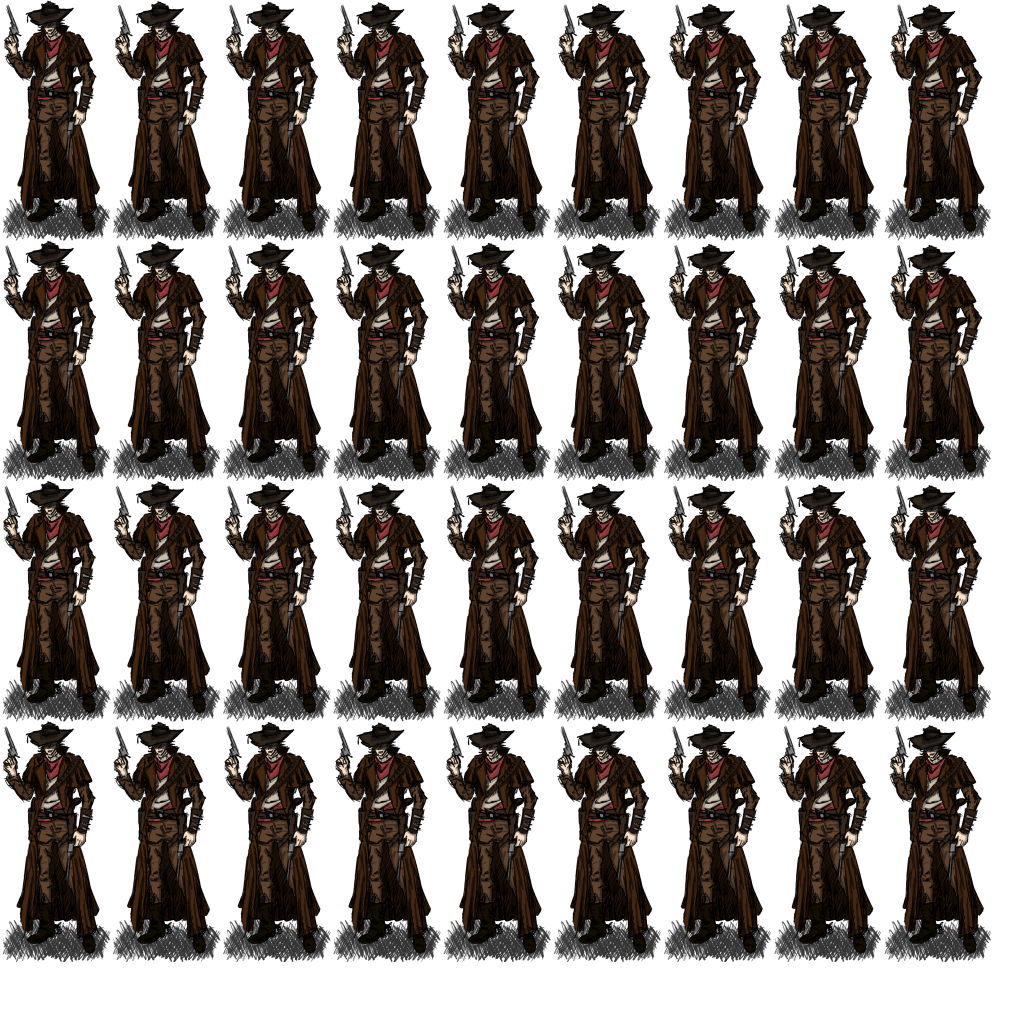
\includegraphics[scale=0.5]{example_animation_atlas.png}
    \caption{Beispiel für Animations-Atlas in 20\% der Original-Auflösung}
\end{figure}

Die \inlineKotlin{DeferredFrameAnimation} Klasse implementiert die Lade-Logik für Animationen.
Beim Erstellen einer Instanz dieser Klasse wird eine Nachricht an der ServiceThread geschickt, die diesem befiehlt,
den Atlas mit den Frames er Animation zu laden.
Der ServiceThread startet eine Coroutine auf einem gesonderten Thread nur für Animation, um zu verhindern, dass das
Laden der Animation das Laden anderer Ressourcen, die zeitkritisch sein könnten, blockiert.
Während die eigentliche Animation geladen wird, rendert DeferredFameAnimation ein statisches Preview-Bild,
typischerweise der erste Frame der Animation, um die Ladezeit zu überbrücken.
Nachdem das asynchrone Laden des Atlases abgeschlossen ist, müssen die Texturen dieses Atlases
auf dem Main-Thread zur GPU hochgeladen werden.
Durch die Größe der Texturen führt das zu merkbaren Lag.
Um das zumindest weniger auffällig zu machen, passiert der Upload der Texturen zwischen Render-Zyklen und mit 100ms
Zeitverzögerung zwischen Uploads.

% resets author
\renewcommand{\kapitelautor}{}
